\setcounter{section}{1}
\section{CĂN BẬC BA}
\subsection{Trọng tâm kiến thức}
\begin{tomtat}
\subsubsection{Căn bậc ba}
\begin{boxdn}
	Căn bậc ba của số thực $a$ là số thực $x$ thỏa mãn $x^3=a$.
\end{boxdn}
\begin{note}
	Mỗi số $a$ đều có duy nhất một căn bậc ba. Căn bậc ba của số $a$ được kí hiệu là $\sqrt[3]{a}$. Trong kí hiệu $\sqrt[3]{a}$, số $3$ được gọi là \textit{chỉ số} của căn. Phép tìm căn bậc ba của một số gọi là \textit{phép khai căn bậc ba}.
\end{note}
\begin{nx}
	Từ định nghĩa căn bậc ba, ta có $\left(\sqrt[3]{a}\right)^3=\sqrt[3]{a^3}=a$ với mọi số thực $a$.
\end{nx}
\subsubsection{Căn thức bậc ba}
\begin{boxdn}
	Căn thức bậc ba là biểu thức có dạng $\sqrt[3]{A}$, trong đó $A$ là một biểu thức đại số.
\end{boxdn}
\begin{note}
	\begin{itemize}
	\item Tương tự căn bậc ba của một số, ta cũng có $\left(\sqrt[3]{A}\right)^3=\sqrt[3]{A^3}=A$ ($A$ là một biểu thức).
	\item Để tính giá trị của $\sqrt[3]{A}$ tại những giá trị cho trước của biến, ta thay các giá trị cho trước của biến vào căn thức rồi tính giá trị của biểu thức số nhận được.
	\end{itemize}
\end{note}
\end{tomtat}
%%%%%%%%%%%%%%%%%%%%
\subsection{Các dạng bài tập}
%=================
\begin{dang}{Tính căn bậc ba, căn thức bậc ba}
\end{dang}
%%==========Ví dụ 2
\begin{vd}
	Không dùng MTCT, tính:
	\begin{listEX}[4]
	\item $\sqrt[3]{1\,000}$;
	\item $\sqrt[3]{-0{,}064}$;
	\item $\sqrt[3]{-8}$;
	\item $\sqrt[3]{0{,}125}$;
	\item $\sqrt[3]{125}$;
	\item $\sqrt[3]{0{,}008}$;
	\item $\sqrt[3]{216}$;
	\item $\sqrt[3]{729}$	;
	\item $\sqrt[3]{1331}$;
	\item $\sqrt[3]{-343}$;
	\item $\sqrt[3]{-1728}$;
	\item $\sqrt[3]{-27}$.
	\end{listEX}
	\loigiai{
	\begin{listEX}[3]
	\item $\sqrt[3]{1\,000}=10$.
	\item $\sqrt[3]{-0{,}064}=-0{,}4$.
	\item $\sqrt[3]{-8}=-2$.
	\item $\sqrt[3]{0{,}125}=0{,}5$.
	\item $\sqrt[3]{125}=\sqrt[3]{5^3}=5$.
	\item $\sqrt[3]{0{,}008}=\sqrt[3]{(0{,}2)^3}=0{,}2$.
	\item $\sqrt[3]{216}=\sqrt[3]{6^3}= 6$.
	\item $\sqrt[3]{729}=\sqrt[3]{9^3}= 9$.
	\item $\sqrt[3]{1331}=\sqrt[3]{11^3}= 11$.
	\item $\sqrt[3]{-343}=\sqrt[3]{( - 7)^3}= - 7$.
	\item $\sqrt[3]{-1728}=\sqrt[3]{( - 12)^3}= - 12$.
	\item $\sqrt[3]{-27}=\sqrt[3]{(-3)^3}=-3$.
	\end{listEX}
	}
\end{vd}
%%==========Ví dụ 3
\begin{vd}%[9D1Y9]
	Không dùng MTCT, tính:
	\begin{listEX}[4]
	\item $\sqrt[3]{\dfrac{8}{27}}$;
	\item $\sqrt[3]{ - \dfrac{125}{512}}$;
	\item $\sqrt[3]{\dfrac{1}{125}}$;
	\item $\sqrt[3]{\dfrac{-8}{125}}$.
	\end{listEX}
	\loigiai
	{
	\begin{listEX}[2]
	\item $\sqrt[3]{\dfrac{8}{27}}=\sqrt[3]{\left(\dfrac{2}{3}\right)^3}=\dfrac{2}{3}$.
	\item $\sqrt[3]{ - \dfrac{125}{512}}=\sqrt[3]{\left( - \dfrac{5}{8}\right)^3}= - \dfrac{5}{8}$.
	\item $\sqrt[3]{\dfrac{1}{125}}=\sqrt[3]{\left( \dfrac{1}{5}\right)^3}=\dfrac{1}{5}$.
	\item $\sqrt[3]{\dfrac{-8}{125}}=\sqrt[3]{\left(-\dfrac{2}{5}\right)^3}=-\dfrac{2}{5}$.
	\end{listEX}
	}
\end{vd}
%%==========Ví dụ 4
\begin{vd}
	\begin{enumerate}
	\item Tính giá trị của căn thức $\sqrt[3]{5x-1}$ tại $x=0$ và tại $x=-1{,}4$.
	\item Tính giá trị của căn thức $\sqrt[3]{2x+5}$ tại $x=60$ và tại $x=-6{,}5$.
	\end{enumerate}
	\loigiai{
	\begin{enumerate}
	\item 
	Với $x=0$ ta có $\sqrt[3]{5\cdot 0-1}=\sqrt[3]{-1}=\sqrt[3]{(-1)^3}=-1$.\\
	Với $x=-1{,}4$ ta có $\sqrt[3]{5\cdot \left(-1{,}4\right)-1}=\sqrt[3]{-8}=\sqrt[3]{(-2)^3}=-2$.
	\item 
	Với $x=60$ ta có $\sqrt[3]{2\cdot 60+5}=\sqrt[3]{125}=\sqrt[3]{5^3}=5$.\\
	Với $x=-6{,}5$ ta có $\sqrt[3]{2\cdot \left(-6{,}5\right)+5}=\sqrt[3]{-8}=\sqrt[3]{(-2)^3}=-2$.
	\end{enumerate}
	}
\end{vd}
%%==========Ví dụ 5
\begin{vd}
	Sử dụng máy tính cầm tay, tính các căn bậc ba sau và làm tròn kết quả với độ chính xác $0{,}005$.
	\begin{listEX}[2]
	\item $\sqrt[3]{45}$;
	\item $\sqrt[3]{3{,}25}$.
	\end{listEX}
	\loigiai{
	\begin{listEX}
	\item Bấm các phím \shiftk\sqrtk\fourk\fivek, màn hình hiện kết quả $3{,}556893304$.\\
	Làm tròn kết quả với độ chính xác $0{,}005$ ta được $\sqrt[3]{45}\approx 3{,}56$.
	\item Bấm các phím \shiftk\sqrtk\threek\dotk\twok\fivek, màn hình hiện kết quả $1{,}481248034$.\\
	Làm tròn kết quả đến chữ số thập phân thứ hai ta được $\sqrt[3]{3{,}25}\approx 1{,}48$.
	\end{listEX}
	}
\end{vd}
%%==========Ví dụ 6
\begin{vd}
	Sử dụng MTCT, tìm căn bậc ba của các số sau (kết quả làm tròn đến chữ số thập phân thứ ba)
	\begin{enumEX}{6}
	\item $15$;
	\item $-12{,}37$;
	\item $25$;
	\item $-100$;
	\item $8{,}5$;
	\item $\dfrac{1}{5}$.
	\end{enumEX}
	\loigiai{
	\begin{enumerate}
	\item Để tính $\sqrt[3]{15}$, ấn liên tiếp các phím 
	\key{q}\key{s}\key{1}\key{5}\key{=} ta được kết quả $2{,}466212074$.\\
	Từ đó, $\sqrt[3]{15}\approx 2{,}466$ (kết quả làm tròn đến chữ số thập phân thứ ba).
	\item Để tính $\sqrt[3]{-12{,}37}$, ấn liên tiếp các phím 
	\key{q}\key{s}\key{z}\key{1}\key{2}\key{.}\key{3}\key{7}\key{=} ta được kết quả $-2{,}312720943$.\\
	Từ đó, $\sqrt[3]{-12{,}37}\approx -2{,}313$ (kết quả làm tròn đến chữ số thập phân thứ ba).
	\item Để tính $\sqrt[3]{25}$, ấn liên tiếp các phím 
	\key{q}\key{s}\key{2}\key{5}\key{=} ta được kết quả $2{,}9240177$.\\
	Từ đó, $\sqrt[3]{25}\approx 2{,}924$ (kết quả làm tròn đến chữ số thập phân thứ ba).
	\item Để tính $\sqrt[3]{-100}$, ấn liên tiếp các phím 
	\key{q}\key{s}\key{z}\key{1}\key{0}\key{0}\key{=} ta được kết quả $-4{,}641589$.\\
	Từ đó, $\sqrt[3]{-100}\approx -4{,}642$ (kết quả làm tròn đến chữ số thập phân thứ ba).
	\item Để tính $\sqrt[3]{8{,}5}$, ấn liên tiếp các phím 
	\key{q}\key{s}\key{8}\key{.}\key{5}\key{=} ta được kết quả $2{,}0408276$.\\
	Từ đó, $\sqrt[3]{8{,}5}\approx 2{,}041$ (kết quả làm tròn đến chữ số thập phân thứ ba).
	\item Để tính $\sqrt[3]{\dfrac{1}{5}}$, ấn liên tiếp các phím 
	\key{q}\key{s}\key{1}\key{a}\key{5}\key{=} ta được kết quả $0{,}58480355$.\\
	Từ đó, $\sqrt[3]{\dfrac{1}{5}}\approx 0{,}485$ (kết quả làm tròn đến chữ số thập phân thứ ba).
	\end{enumerate}
	}
\end{vd}
%%==========Ví dụ 7
\begin{vd}
	Cho biểu thức $P=\sqrt[3]{3x-2}$. Tính giá trị của $P$ khi $x=3$ và khi $x=-2$ (kết quả làm tròn đến chữ số thập phân thứ ba).
	\loigiai{
	\begin{itemize}
	\item Với $x=3$, ta có $P=\sqrt[3]{3\cdot 3-2}=\sqrt[3]{7}\approx 1{,}913$;
	\item Với $x=-2$, ta có $P=\sqrt[3]{3\cdot (-2)-2}=\sqrt[3]{-8}=-2$.
	\end{itemize}
	}
\end{vd}
%%==========Ví dụ 8
\begin{vd}
	Cho biểu thức $Q=\sqrt[3]{3x^2}$. Tính giá trị của $Q$ khi $x=2$ và khi $x=-3$ (kết quả làm tròn đến chữ số thập phân thứ hai).
	\loigiai{
	\begin{itemize}
	\item Với $x=2$, ta có $Q=\sqrt[3]{3\cdot 2^2}=\sqrt[3]{12}\approx 2{,}29$;
	\item Với $x=-3$, ta có $Q=\sqrt[3]{3\cdot (-3)^2}=\sqrt[3]{27}=3$.
	\end{itemize}
	}
\end{vd}
%====================
\begin{dang}{So sánh}
\end{dang}
%%==========Ví dụ 9
\begin{vd}
	So sánh
	\begin{enumEX}{2}
	\item $\sqrt[3]{-11{,}35}$ và $\sqrt[3]{-13{,}12}$;
	\item $3$ và $\sqrt[3]{27\dfrac{1}{4}}$;
	\item $7 \text{ và } \sqrt[3]{345}$;
	\item $2\sqrt[3]{6} \text{ và } 3\sqrt[3]{2}$.
	\end{enumEX}
	\loigiai{
	\begin{listEX}
	\item Do $-11{,}35>-13{,}12$ nên $\sqrt[3]{-11{,}35}>\sqrt[3]{-13{,}12}$.
	\item Ta có $3=\sqrt[3]{27}$. Do $27<27\dfrac{1}{4}$ nên $\sqrt[3]{27}<\sqrt[3]{27\dfrac{1}{4}}$ hay $3<\sqrt[3]{27\dfrac{1}{4}}$.
	\item Ta có $7 =\sqrt[3]{343}$. Do $343<345$ nên $\sqrt[3]{343}<\sqrt[3]{345}$.
	\item Ta có $2\sqrt[3]{6}=\sqrt[3]{8\cdot6}=\sqrt[3]{48}$; $3\sqrt[3]{2}=\sqrt[3]{27\cdot 2}=\sqrt[3]{54}$.
	Do $48 < 54$ nên $2\sqrt[3]{6}< 3\sqrt[3]{2}$.
	\end{listEX} 
	}
\end{vd}
%%==========Ví dụ 10
\begin{vd}%[9D1B9]
	So sánh \begin{listEX}[2]
	\item $\dfrac{2}{3}\sqrt[3]{18}\text{ và }\dfrac{3}{4}\sqrt[3]{12}$;
	\item $\sqrt[3]{130} + 1\text{ và } 3\sqrt[3]{12} - 1$
	\end{listEX}
	\loigiai
	{
	\begin{enumerate}
	\item Ta có \allowdisplaybreaks \begin{align*}
	\begin{array}{l}
	{\dfrac{2}{3}\sqrt[3]{18}=\sqrt[3]{\left(\dfrac{2}{3}\right)^3\cdot 18}=\sqrt[3]{\dfrac{16}{3}}=\sqrt[3]{5\dfrac{1}{3}}}.\\
	{\dfrac{3}{4}\sqrt[3]{12}=\sqrt[3]{\left(\dfrac{3}{4}\right)^3\cdot 12}=\sqrt[3]{\dfrac{81}{16}}=\sqrt[3]{5\dfrac{1}{16}}}
	\end{array}.
	\end{align*}
	$\text{ Vì }	5\dfrac{1}{3}> 5\dfrac{1}{16}\text{ nên }\dfrac{2}{3}\sqrt[3]{18}>\dfrac{3}{4}\sqrt[3]{12}$.
	\item Ta có 
	\allowdisplaybreaks \begin{align*}
	&\sqrt[3]{130} + 1>\sqrt[3]{1\sqrt{15}} + 1=5 + 1=6;
	\\ &3\sqrt[3]{12} - 1=\sqrt[3]{27.12} - 1=\sqrt[3]{324} - 1<\sqrt[3]{343} - 1=7 - 1=6 .
	\end{align*}
	Vậy $\sqrt[3]{130} + 1>3\sqrt[3]{12} - 1$.
	\end{enumerate}
	}
\end{vd}
%%==========Ví dụ 11
\begin{vd}%[9D1B9]
	Cho $a<0$, hỏi số nào lớn hơn trong hai số $\sqrt[3]{2a}$ và $\sqrt[3]{3a}$?
	\loigiai
	{Ta có $2<3$ suy ra $2a>3a$ (vì $a<0$).\\ Do đó $\sqrt[3]{2a}>\sqrt[3]{3a}$.
	}
\end{vd}
%%%%%%%%%%%%%
\begin{dang}{Tính giá trị, rút gọn biểu thức chứa căn bậc ba}
	\begin{note}
	Với mọi $A$, $B$ ta có
	\begin{enumEX}[\itemCI]{2}
	\item $\sqrt[3]{A}:\sqrt[3]{B}=\sqrt[3]{A:B}$.
	\item 
	$\sqrt[3]{A}\cdot\sqrt[3]{B}=\sqrt[3]{AB}$.
	\end{enumEX}
	\end{note}
\end{dang}
%%==========Ví dụ 12
\begin{vd}
	Tính giá trị của biểu thức
	\begin{enumEX}{2}
	\item $A=\sqrt[3]{8000}+\sqrt[3]{0{,}125}$;
	\item $B=\sqrt[3]{12^3}-\sqrt[3]{(-11)^3}$;
	\item $C=\left(\sqrt[3]{4}\right)^3+\left(\sqrt[3]{-5}\right)^3$;
	\item $D=\sqrt[3]{1000} +\left(\sqrt[3]{8{,}9}\right)^3$.
	\end{enumEX}
	\loigiai{
	\begin{enumEX}{2}
	\item Ta có\\
	$\begin{aligned}
	A &= \sqrt[3]{8000}+\sqrt[3]{0{,}125}\\
	&= \sqrt[3]{20^3}+\sqrt[3]{(0{,}5)^3}\\
	&= 20+0{,}5\\
	&= 20{,}5.
	\end{aligned}$
	\item Ta có\\
	$\begin{aligned}
	B &= \sqrt[3]{12^3}-\sqrt[3]{(-11)^3}\\
	&= 12+(-11)\\
	&= -1.
	\end{aligned}$
	\item Ta có\\
	$\begin{aligned}
	C &= \left(\sqrt[3]{4}\right)^3+\left(\sqrt[3]{-5}\right)^3\\
	&= 4+(-5)\\
	&= 1.
	\end{aligned}$
	\item Ta có\\
	$\begin{aligned}[t]
	D&=\sqrt[3]{1000} +\left(\sqrt[3]{8{,}9}\right)^3\\
	&=\sqrt[3]{10^3}\cdot +8{,}9\\
	&=10+8{,}9=18{,}9.
	\end{aligned}$
	\end{enumEX}
	}
\end{vd}
%%==========Ví dụ 13
\begin{vd}%[9D1B9]
	Rút gọn các biểu thức
	\begin{listEX}[2]
	\item $\sqrt[3]{8} + \sqrt[3]{ - 27} + \sqrt[3]{ - 64}$;
	\item $\sqrt[3]{54} - \sqrt[3]{ - 16} + \sqrt[3]{128}$;
	\item $\sqrt[3]{16}\cdot\sqrt[3]{13,5} - \sqrt[3]{120}:\sqrt[3]{15}$;
	\item $(\sqrt[3]{2} + 1)(\sqrt[3]{4} - \sqrt[3]{2} + 1)$;
	\item $(\sqrt[3]{5} + 1)^3 - 3\sqrt[3]{5}(\sqrt[3]{5} + 1)$;
	\item $(\sqrt[3]{4} - \sqrt[3]{2})^3 + 6\sqrt[3]{2}(\sqrt[3]{2} - 1)$.
	\end{listEX}
	\loigiai{
	\begin{listEX}[1]
	\item $\sqrt[3]{8} + \sqrt[3]{ - 27} + \sqrt[3]{ - 64}=2 + ( - 3) + ( - 4)= - 5$.
	\item $\sqrt[3]{54} - \sqrt[3]{ - 16} + \sqrt[3]{128}=\sqrt[3]{3^3\cdot 2} - \sqrt[3]{( - 2)^3\cdot 2} + \sqrt[3]{4^3\cdot 2}=3\sqrt[3]{2} + 2\sqrt[3]{2} + 4\sqrt[3]{2}=9\sqrt[3]{2}$.
	\item \allowdisplaybreaks $\begin{aligned}[t]
	\sqrt[3]{16}\cdot\sqrt[3]{13,5} - \sqrt[3]{120}:\sqrt[3]{15}
	=\sqrt[3]{16.13,5} - \sqrt[3]{120 : 15}
	=\sqrt[3]{216} - \sqrt[3]{8}
	=6 - 2=4.
	\end{aligned}$ 
	\item 
	\allowdisplaybreaks 
	$\begin{aligned}[t]
	(\sqrt[3]{2} + 1)(\sqrt[3]{4} - \sqrt[3]{2} + 1)
	=\sqrt[3]{8} - \sqrt[3]{4} + \sqrt[3]{2} + \sqrt[3]{4} - \sqrt[3]{2} + 1
	=2 + 1=3.
	\end{aligned}$ 
	\item $\left(\sqrt[3]{5} + 1\right)^3 - 3\sqrt[3]{5}\left(\sqrt[3]{5} + 1\right)=5 + 3\sqrt[3]{25} + 3\sqrt[3]{5} + 1 - 3\sqrt[3]{25} - 3\sqrt[3]{5}=6$.
	\item 
	\allowdisplaybreaks 
	$\begin{aligned}[t]
	\left(\sqrt[3]{4} - \sqrt[3]{2}\right)^3 + 6\sqrt[3]{2}\left(\sqrt[3]{2} - 1\right)=\,&4 - 3\sqrt[3]{32} + 3\sqrt[3]{16} - 2 + 6\sqrt[3]{4} - 6\sqrt[3]{2}\\
	=\,&4 - 6\sqrt[3]{4} + 6\sqrt[3]{2} - 2 + 6\sqrt[3]{4} - 6\sqrt[3]{2}=2.
	\end{aligned}$
	\end{listEX}
	}
\end{vd}
%%==========Ví dụ 14
\begin{vd}%[9D1K9]
	Tính $A=\sqrt[3]{\sqrt{5} + 2} - \sqrt[3]{\sqrt{5} - 2}$
	\loigiai
	{
	Để tính giá trị của $A$, ta tính $A^3$ sau đó suy ra $A$.\\ 
	Bạn nên nhớ hằng đẳng thức $(a - b)^3=a^3 - b^3 - 3a b(a - b)$.\\ 
	Ta có
	\begin{align*}
	A^3&=\left(\sqrt[3]{\sqrt{5} + 2} - \sqrt[3]{\sqrt{5} - 2}\right)^3\\
	&=(\sqrt{5} + 2) - (\sqrt{5} - 2) - 3\sqrt[3]{(\sqrt{5} + 2)(\sqrt{5} - 2)}\cdot\left(\sqrt[3]{\sqrt{5} + 2} - \sqrt[3]{\sqrt{5} - 2}\right)
	\end{align*}
	$\Rightarrow A^3=4 - 3A$
	$\begin{aligned}[t]
	\Rightarrow A^3 + 3A - 4=0 &\Leftrightarrow(A - 1)\left(A^2 + A + 4\right)=0\\
	&\Leftrightarrow A - 1=0~\left(\text{vì }A^2 + A + 4>0\right)\\
	&\Leftrightarrow A=1.
	\end{aligned}$\\
	Vậy $A=1$.
	}
\end{vd}
%%==========Ví dụ 15
\begin{vd}%[9D1B9]
	Rút gọn biểu thức 
	\begin{listEX}[2]
	\item $\sqrt[3]{x^3 + 1 + 3x(x + 1)}$;
	\item $\dfrac{x + 1}{\sqrt[3]{x^2} - \sqrt[3]{x} + 1}$;
	\item $\sqrt[3]{x^3-3x^2+3x-1}$;
	\item $-x+5+\sqrt[3]{x^3+3x^2+3x+1}$.
	\end{listEX}
	\loigiai
	{
	\begin{enumerate}
	\item $\sqrt[3]{x^3 + 1 + 3x(x + 1)}=\sqrt[3]{(x + 1)^3}=x + 1$.
	\item $\dfrac{x + 1}{\sqrt[3]{x^2} - \sqrt[3]{x} + 1}=\dfrac{(\sqrt[3]{x} + 1)\left(\sqrt[3]{x^2} - \sqrt[3]{x} + 1\right)}{\sqrt[3]{x^2} - \sqrt[3]{x} + 1}=\sqrt[3]{x} + 1$.
	\item $\sqrt[3]{x^3-3x^2+3x-1}=\sqrt[3]{(x-1)^3}=x-1$.
	\item $-x+5+\sqrt[3]{x^3+3x^2+3x+1}=-x+5+\sqrt[3]{(x+1)^3}=-x+5+x+1=6$.
	\end{enumerate}
	}
\end{vd}
%===================
\begin{dang}{Bài toán thực tế}
\end{dang}
\begin{vd}
	Có hai khối bê tông hình lập phương A và B có thể tích lần lượt là $8$ dm$^3$ và $15$ dm$^3$ (xem hình vẽ).
	\begin{center}	
	\begin{tikzpicture}
	\def\a{2}
	\path 	(0:0) coordinate (A)
	++(0:\a) coordinate (D)
	++(-130:\a/2) coordinate (C)
	($(A)+(C)-(D)$) coordinate (B)
	($(A)+(90:\a)$) coordinate (A')
	($(B)+(90:\a)$) coordinate (B')
	($(C)+(90:\a)$) coordinate (C')
	($(D)+(90:\a)$) coordinate (D');
	\draw[dashed,thick] 	(B)--(A)--(D)	(A)--(A');
	\draw[thick] 	(C)--(C') 	(D)--(D') 	(B)--(B') 	
	(B)--(C)node[pos=0.5,sloped,below=8pt]{\textbf{Khối lập phương A}}--(D) (A')--(B')--(C')--(D')--cycle;	
	\end{tikzpicture}\hspace{2cm}
	\begin{tikzpicture}
	\def\a{2.6}
	\path 	(0:0) coordinate (A)
	++(0:\a) coordinate (D)
	++(-130:\a/2) coordinate (C)
	($(A)+(C)-(D)$) coordinate (B)
	($(A)+(90:\a)$) coordinate (A')
	($(B)+(90:\a)$) coordinate (B')
	($(C)+(90:\a)$) coordinate (C')
	($(D)+(90:\a)$) coordinate (D');
	\draw[dashed,thick] 	(B)--(A)--(D)	(A)--(A');
	\draw[thick] 	(C)--(C') 	(D)--(D') 	(B)--(B') 	
	(B)--(C)node[pos=0.5,sloped,below=8pt]{\textbf{Khối lập phương B}}--(D) (A')--(B')--(C')--(D')--cycle;
	\end{tikzpicture}
	\end{center}
	\begin{enumerate}
	\item Tính độ dài cạnh của khối bê tông A.
	\item Gọi $x$ (dm) là độ dài cạnh của khối bê tông B. Thay dấu $\fbox{?}$ bằng số thích hợp để có đẳng thức $x^3=\fbox{?}$
	\end{enumerate}
	\loigiai{
	\begin{enumerate}
	\item Gọi $a$ (cm) là độ dài cạnh của khối bê tông A, với $a>0$.\\
	Ta có $a^3=8$ hay $a^3=2^3$ suy ra $a=2$ (cm). \\
	Vậy độ dài cạnh của khối bê tông A là $a=2$ (cm).
	\item Gọi $x$ (dm) là độ dài cạnh của khối bê tông B, với $x>0$.\\
	Ta có $x^3=15$ suy ra $x=\sqrt[3]{15}\approx 2{,}466$ (cm).
	\end{enumerate}
	}
\end{vd}
%%==========Ví dụ 1
\begin{vd}
	Dùng định luật thứ ba của Kepler về sự chuyển động của các hành tinh trong hệ Mặt Trời cho biết khoảng cách trung bình $d$ (triệu dặm) từ một hành tinh quay xung quanh Mặt Trời đến Mặt Trời được tính bởi công thức $d=\sqrt[3]{6r^2}$ với $t$ (ngày Trái Đất) là thời gian hành tinh đó quay quanh Mặt Trời đúng một vòng (\textit{Nguồn: https://vi.wikipedia.org}).
	\begin{center}
	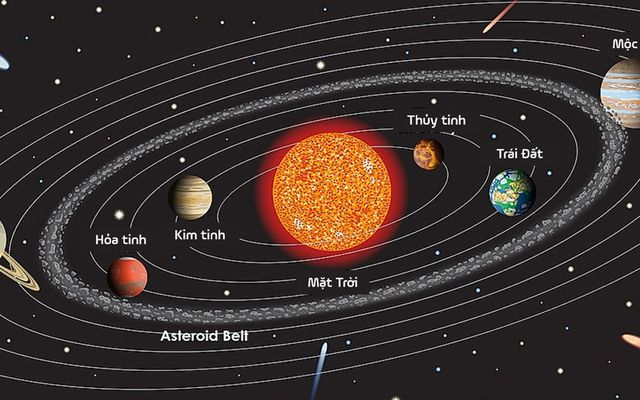
\includegraphics[scale=0.4]{images/9C3-1-1}\\
	\end{center}
	\begin{center}
	\color{blue}{Hệ Mặt Trời}
	\end{center}
	\begin{enumerate}
	\item Trái Đất quay một vòng quanh Mặt Trời trong khoảng $365$ ngày Trái Đất. Hỏi khoảng cách trung bình giữa Trái Đất và Mặt Trời là bao nhiêu triệu kilômét (làm tròn kết quả đến hàng phần mười)? Biết $1$ dặm $= 1{,}609344$ km.
	\item Một năm Sao Hỏa dài bằng $687$ ngày trên Trái Đất, nghĩa là Sao Hỏa quay xung quanh Mặt trời đúng một vòng với thời gian bằng $687$ ngày Trái Đất. Hỏi khoảng cách trung bình giữa Sao Hỏa và Mặt Trời là bao nhiêu triệu kilômét (làm tròn kết quả đến hàng phần mười)?
	\end{enumerate}
	\loigiai{
	\begin{enumerate}
	\item Thay $t=365$ vào công thức $d=\sqrt[3]{6t^2}$, ta có
	\begin{center}
	$d=\sqrt[3]{6\cdot 365^2}=\sqrt[3]{799\,350}\approx 92{,}807$ (triệu dặm).
	\end{center}
	Đổi $92{,}807$ triệu dặm $\approx 149{,}4$ triệu km.\\
	Vậy khoảng cách trung bình giữa Trái Đất và Mặt Trời là khoảng $149,4$ triệu km.
	\item Thay $t=687$ vào công thức $d=\sqrt[3]{6t^2}$, ta có
	\begin{center}
	$d=\sqrt[3]{6\cdot 687^2}=\sqrt[3]{2\,831\,814}\approx 141{,}4787$ (triệu dặm).
	\end{center}
	Đổi $141{,}478$ triệu dặm $\approx 227{,}7$ triệu km.\\
	Vậy khoảng cách trung bình giữa Sao Hỏa và Mặt Trời là khoảng $227{,}7$ triệu km.
	\end{enumerate}	
	}
\end{vd}
%%=====Bài 7
\begin{vd}
	Chiều cao ngang vai của một con voi đực ở châu Phi là $h$ (cm) có thể được tính xấp xỉ bằng công thức $h=62,5\sqrt[3]{t}+75,8$ với $t$ là tuổi con voi tính theo năm (Nguồn: J.Libby, Math for Real Life: Teaching and Practical Uses for Algebra, McFarland, năm 2017).
	\begin{listEX}[1]
	\item Một con voi đực $8$ tuổi thì có chiều cao ngang vai là bao nhiêu centimet?
	\item Nếu một con voi đực có chiều cao ngang vai là $205$ cm thì con voi đó bao nhiêu tuổi (làm tròn kết quả đến hàng đơn vị)?
	\end{listEX}
	\loigiai{
	\begin{listEX}[1]
	\item Một con voi đực $8$ tuổi thì có chiều cao ngang vai là \[62,5 \sqrt[3]{8}+75,8=200,8 \text{ (centimet)}.\]
	\item Nếu một con voi đực có chiều cao ngang vai là $205$ cm thì 
	\begin{eqnarray*}
	205&=&62,5 \sqrt[3]{t}+75,8\\
	\sqrt[3]{t}&=&2,0672\\
	t &= &2{,}0672^3\\
	t &= &8{,}733798504.
	\end{eqnarray*}
	Vậy con voi đó khoảng $9$ tuổi.
	\end{listEX}
	}
\end{vd}
%%%%%%%%%%%%%%%%%%%%
\subsection{Bài tập vận dụng}
%%==========Bài 1
\begin{bt}
	Tìm căn bậc ba của mỗi số sau
	\begin{enumEX}{4}
	\item $-64$;
	\item $27\,000$;
	\item $-0{,}125$;
	\item $3\dfrac{3}{8}$.
	\end{enumEX}
	\loigiai{
	\begin{enumEX}{1}
	\item Ta có $(-4)^3=-64$ suy ra $\sqrt[3]{-64}=-4$.
	\item Ta có $30^3=27\,000$ suy ra $\sqrt[3]{27\,000}=30$.
	\item Ta có $(-0{,}5)^3=-0{,}125$ suy ra $\sqrt[3]{-0{,}125}=-0{,}5$.
	\item Ta có $3\dfrac{3}{8}=\dfrac{27}{8}=\left(\dfrac{3}{2}\right)^3$ suy ra $\sqrt[3]{3\dfrac{3}{8}}=\dfrac{3}{2}$.
	\end{enumEX}
	}
\end{bt}
%%==========Bài 2
\begin{bt}
	Tìm căn bậc ba của:
	\begin{listEX}[4]
	\item $1331$;
	\item $-27$;
	\item $-0{,}216$;
	\item $\dfrac{8}{343}$.
	\end{listEX}
	\loigiai{
	\begin{listEX}[2]
	\item $\sqrt[3]{1331}=\sqrt[3]{11^3}=11$;
	\item $\sqrt[3]{-27}=\sqrt[3]{(-3)^3}=-3$;
	\item $\sqrt[3]{-0{,}216}=\sqrt[3]{(-0{,}6)^3}=-0{,}6$;
	\item $\sqrt[3]{\dfrac{8}{343}}=\sqrt[3]{\left(\dfrac{2}{7}\right)^3}=\dfrac{2}{7}\cdot$
	\end{listEX}
	}
\end{bt}
%%==========Bài 3
\begin{bt}
	Tính
	\begin{listEX}[4]
	\item $\sqrt[3]{216}$;
	\item $\sqrt[3]{-512}$;
	\item $\sqrt[3]{-0{,}001}$;
	\item $\sqrt[3]{1{,}331}$.
	\end{listEX}
	\loigiai
	{
	\begin{listEX}[2]
	\item $\sqrt[3]{216}=\sqrt[3]{6^3}=6$;
	\item $\sqrt[3]{-512}=\sqrt[3]{(-8)^3}=-8$;
	\item $\sqrt[3]{-0{,}001}=\sqrt[3]{(-0{,}1)^3}=-0{,}1$;
	\item $\sqrt[3]{1{,}331}=\sqrt[3]{(1{,}1)^3}=1{,}1$.
	\end{listEX}
	}
\end{bt}
%%==========Bài 4
\begin{bt}
	Tính
	\begin{enumEX}{4}
	\item $\sqrt[3]{0{,}001}$;
	\item $\sqrt[3]{-\dfrac{1}{64}}$;
	\item $-\sqrt[3]{11^3}$;
	\item $\left(\sqrt[3]{-216}\right)^3$.
	\end{enumEX}
	\loigiai{
	\begin{enumEX}{2}
	\item Ta có $\sqrt[3]{0{,}001}=\sqrt[3]{(0{,}1)^3}=0{,}1$.
	\item Ta có $\sqrt[3]{-\dfrac{1}{64}}=\sqrt[3]{\left(-\dfrac{1}{4}\right)^3}=-\dfrac{1}{4}$
	\item Ta có $-\sqrt[3]{11^3}=11$.
	\item Ta có $\left(\sqrt[3]{-216}\right)^3=-216$.
	\end{enumEX}
	}
\end{bt}
%%==========Bài 5
\begin{bt}
	Hoàn thành bảng sau vào vở
	\begin{center}
	\begin{tabular}{*{11}{|c}|}
	\hline
	$a$ & $1$ & $8$ & $27$ & $64$ & $?$ & $?$ & $?$ & $?$ & $?$ & $?$\\
	\hline
	$\sqrt[3]{a}$ & $?$ & $?$ & $?$ & $?$ & $5$ & $6$ & $7$ & $8$ & $9$ & $10$ \\
	\hline
	\end{tabular}
	\end{center}
	\loigiai{
	\begin{center}
	\begin{tabular}{*{11}{|c}|}
	\hline
	$a$ & $1$ & $8$ & $27$ & $64$ & \color{red}$125$ & \color{red}$216$ & \color{red}$343$ & \color{red}$512$ & \color{red}$729$ & \color{red}$1000$\\
	\hline
	$\sqrt[3]{a}$ & \color{red}$1$ & \color{red}$2$ & \color{red}$3$ & \color{red}$4$ & $5$ & $6$ & $7$ & $8$ & $9$ & $10$ \\
	\hline
	\end{tabular}
	\end{center}
	}
\end{bt}
%%==========Bài 6
\begin{bt}
	Tính giá trị của biểu thức $P=\sqrt[3]{64n}$ khi $n=1$; $n=-1$; $n=\dfrac{1}{125}$.
	\loigiai{
	\begin{itemize}
	\item Với $n=1$, ta có $P=\sqrt[3]{64\cdot 1}=\sqrt[3]{64}=\sqrt[3]{4^3}=4$.
	\item Với $n=-1$, ta có $P=\sqrt[3]{64\cdot (-1)}=\sqrt[3]{-64}=\sqrt[3]{(-4)^3}=-4$.
	\item Với $n=\dfrac{1}{125}$, ta có $P=\sqrt[3]{64\cdot \dfrac{1}{125}}=\sqrt[3]{\dfrac{64}{125}}=\sqrt[3]{\left(\dfrac{4}{5}\right)^3}=\dfrac{4}{5}$.
	\end{itemize}
	}
\end{bt}
%%==========Bài 7
\begin{bt}
	Sử dụng MTCT tính các căn bậc ba sau đây (làm tròn kết quả đến chữ số thập phân thứ hai)
	\begin{listEX}[4]
	\item $\sqrt[3]{2{,}1}$ ;
	\item $\sqrt[3]{-18}$ ;
	\item $\sqrt[3]{-28}$ ;
	\item $\sqrt[3]{0{,}35}$
	\end{listEX}
	\loigiai{
	\begin{listEX}
	\item Bấm các phím \shiftk\sqrtk\twok\dotk\onek, màn hình hiện kết quả $1{,}280579165$.\\
	Làm tròn kết quả đến chữ số thập phân thứ hai ta được $\sqrt[3]{2{,}1}\approx 1{,}28$.
	\item Bấm các phím \shiftk\sqrtk\signk\onek\eightk, màn hình hiện kết quả $-2{,}620741394$.\\
	Làm tròn kết quả đến chữ số thập phân thứ hai ta được $\sqrt[3]{-18}\approx -2{,}62$.
	\item Bấm các phím \shiftk\sqrtk\signk\twok\eightk, màn hình hiện kết quả $-3{,}036588972$.\\
	Làm tròn kết quả đến chữ số thập phân thứ hai ta được $\sqrt[3]{-28}\approx -3{,}04$.
	\item Bấm các phím \shiftk\sqrtk\zerok\dotk\threek\fivek, màn hình hiện kết quả $0{,}7047298732$.\\
	Làm tròn kết quả đến chữ số thập phân thứ hai ta được $\sqrt[3]{0{,}35}\approx 0{,}70$.
	\end{listEX}
	}
\end{bt}
%%==========Bài 8
\begin{bt}
	Sử dụng máy tính cầm tay, tính (kết quả làm tròn đến chữ số thập phân thứ ba)
	\begin{enumEX}{3}
	\item $\sqrt[3]{79}$;
	\item $\sqrt[3]{-6{,}23}$;
	\item $\dfrac{\sqrt[3]{19}+\sqrt[3]{20}}{2}$.
	\end{enumEX}
	\loigiai{
	\begin{enumEX}{3}
	\item $\sqrt[3]{79}\approx 4{,}921$;
	\item $\sqrt[3]{-6{,}23}\approx -1{,}840$;
	\item $\dfrac{\sqrt[3]{19}+\sqrt[3]{20}}{2}\approx 2{,}691$.
	\end{enumEX}
	}
\end{bt}
%%==========Bài 9
\begin{bt}
	So sánh:
	\begin{listEX}[2]
	\item $\sqrt[3]{-45}$ và $\sqrt[3]{-50}$;
	\item $-10$ và $\sqrt[3]{-999}$.
	\end{listEX}
	\loigiai{
	\begin{listEX}
	\item Ta có $-45>-50 \Rightarrow \sqrt[3]{-45}>\sqrt[3]{-50}$.
	Vậy $\sqrt[3]{-45}>\sqrt[3]{-50}$.
	\item Ta có $\sqrt[3]{-999}>\sqrt[3]{-1000}=-10$.
	Vậy $-10<\sqrt[3]{-999}$.
	\end{listEX}
	}
\end{bt}
%%==========Bài 10
\begin{bt}
	Tính giá trị của các biểu thức
	\begin{enumEX}{2}
	\item $A=\sqrt[3]{8^3}+\left(\sqrt[3]{-7}\right)^3$;
	\item $B=\sqrt[3]{1\,000\,000}-\sqrt[3]{0{,}027}$.
	\end{enumEX}
	\loigiai{
	\begin{enumEX}{1}
	\item Ta có
	$\begin{aligned}
	A = \sqrt[3]{8^3}+\left(\sqrt[3]{-7}\right)^3
	=8+(-7)=-1.
	\end{aligned}$
	\item Ta có
	$\begin{aligned}
	B =\sqrt[3]{1\,000\,000}-\sqrt[3]{0{,}027}
	=\sqrt[3]{(100)^3}-\sqrt[3]{(0{,}3)^3}
	=100+0{,}3
	=99{,}7.
	\end{aligned}$
	\end{enumEX}
	}
\end{bt}
%%==========Bài 11
\begin{bt}
	Rút gọn các biểu thức sau:
	\begin{listEX}[3]
	\item $\sqrt[3]{\left(1-\sqrt{2}\right)^3}$;
	\item $\sqrt[3]{\left(2\sqrt{2}+1\right)^3}$;
	\item $\left(\sqrt[3]{\sqrt{2}+1}\right)^3$.
	\end{listEX}
	\loigiai{
	\begin{listEX}
	\item $\sqrt[3]{\left(1-\sqrt{2}\right)^3}=1-\sqrt{2}$;
	\item $\sqrt[3]{\left(2\sqrt{2}+1\right)^3}=2\sqrt{2}+1$;
	\item $\left(\sqrt[3]{\sqrt{2}+1}\right)^3=\sqrt{2}+1$.
	\end{listEX}
	}
\end{bt} 
%%==========Bài 12
\begin{bt}
	Rút gọn rồi tính giá trị của biểu thức $\sqrt[3]{27x^3-27x^2+9x-1}$ tại $x=7$.
	\loigiai{
	Ta có $\sqrt[3]{27x^3-27x^2+9x-1}=\sqrt[3]{(3x-1)^3}=3x-1$.\\
	Với $x=7$, giá trị của biểu thức là $3\cdot 7-1=20$.
	}
\end{bt}
%%==========Bài 13
\begin{bt}
	Chứng minh:
	$(\sqrt[3]{2}+1)\left[(\sqrt[3]{2})^2-\sqrt[3]{2}+1\right]=3$.
	\loigiai{
	Ta có $(\sqrt[3]{2}+1)\left[(\sqrt[3]{2})^2-\sqrt[3]{2}+1\right]
	\left(\sqrt[3]{2}\right)^3+1^3=2+1=3$.
	}
\end{bt}
%%==========Bài 14
\begin{bt}
	Tìm $x$ biết
	\begin{enumEX}{4}
	\item $x^3=-27$;
	\item $x^3=\dfrac{64}{125}$;
	\item $\sqrt[3]{x}=8$;
	\item $\sqrt[3]{x}=-0{,}9$.
	\end{enumEX}
	\loigiai{
	\begin{enumEX}{1}
	\item $x^3=-27$ suy ra $x^3=(-3)^3$ suy ra $x=-3$.
	\item $x^3=\dfrac{64}{125}$ suy ra $x^3=\left(\dfrac{4}{5}\right)^3$ suy ra $x=\dfrac{4}{5}$.
	\item $\sqrt[3]{x}=8$ suy ra $\left(\sqrt[3]{x}\right)^3=8^3$ suy ra $x=512$.
	\item $\sqrt[3]{x}=-0{,}9$ suy ra $\left(\sqrt[3]{x}\right)^3=(-0{,}9)^3$ suy ra $x=-0{,}729$.
	\end{enumEX}
	}
\end{bt}
\begin{bt}
	Tìm điều kiện xác định cho mỗi căn thức bậc ba sau
	\begin{listEX}[3]
	\item $\sqrt[3]{3x+2}$
	\item $\sqrt[3]{x^3-1}$
	\item $\sqrt[3]{\dfrac{1}{2-x}}$.
	\end{listEX}
	\loigiai{
	\begin{listEX}[1]
	\item $\sqrt[3]{3x+2}$ xác định với mọi số thực $x$ vì $3x+2$ xác định với mọi số thực $x$.
	\item $\sqrt[3]{x^3-1}$ xác định với mọi số thực $x$ vì $x^3-1$ xác định với mọi số thực $x$.
	\item $\sqrt[3]{\dfrac{1}{2-x}}$ xác định với $x\ne 2$ vì $\dfrac{1}{2-x}$ xác định với $x \ne 2$.
	\end{listEX}
	}
\end{bt}
%%==========Ví dụ 7
\begin{bt}
	Tìm điều kiện xác định cho mỗi căn thức bậc ba sau
	\begin{listEX}[4]
	\item $\sqrt[3]{5 x-11}$;
	\item $\sqrt[3]{x^2+x}$;
	\item $\sqrt[3]{\dfrac{1}{x}}$;
	\item $\sqrt[3]{\dfrac{1}{x-9}}$.
	\end{listEX}
	\loigiai{
	\begin{listEX}
	\item \( \sqrt[3]{5x-11} \) xác định với mọi $x$.
	\item \( \sqrt[3]{x^2+x} \) xác định với mọi $x$.
	\item \( \sqrt[3]{\dfrac{1}{x}} \) xác định khi \( x \neq 0 .\)
	\item \( \sqrt[3]{\dfrac{1}{x-9}} \) xác định khi \( x -9\neq 0 \Rightarrow x\neq 9 .\)
	\end{listEX}
	}
\end{bt}
%%==========Bài 15
\begin{bt}
	Một người thợ muốn làm một thùng tôn hình lập phương có thể tích bằng $730 \mathrm{dm}^3$. Em hãy ước lượng chiều dài cạnh thùng khoảng bao nhiêu dm?
	\loigiai{
	Gọi $x>0$ (dm) là chiều dài cạnh thùng.\\
	Thể tích thùng tôn là $x^3=730$ nên cạnh $x=\sqrt[3]{730}\approx 9$ (dm).
	}
\end{bt}
%%==========Bài 16
\begin{bt}
	Thể tích của một khối bê tông có dạng hình lập phương là khoảng $220\, 348 \mathrm{~cm}^3$. Hỏi độ dài cạnh của khối bê tông đó là bao nhiêu centimét (làm tròn kết quả đến hàng phần mười)?
	\loigiai{
	Gọi $x\, \mathrm{(m)}$ là chiều dài cạnh khối bê tông. \\
	Ta có $x^3=220\, 348 \Rightarrow x=\sqrt[3]{220\, 348}\approx 60{,}4\mathrm{~cm}$. \\
	Vậy khối bê tông có cạnh gần bằng $60{,}4\mathrm{~cm}$.
	}
\end{bt}